\documentclass[10pt,a4paper]{article}
\usepackage[margin=0.8in,top=0.75in,bottom=0.75in]{geometry}
\usepackage[T1]{fontenc}
\usepackage{lmodern,microtype,amsmath,amssymb,booktabs,graphicx,xcolor,tikz,enumitem,array,multirow}
\newcolumntype{P}[1]{>{\raggedright\arraybackslash}p{#1}}
\usepackage[font=small,labelfont=bf,skip=3pt]{caption}
\usepackage[colorlinks=true,linkcolor=blue!50!black,citecolor=blue!50!black,urlcolor=blue!50!black]{hyperref}
\usetikzlibrary{positioning,arrows.meta,shapes.misc}
\setlist{nosep,leftmargin=1.3em}
\setlength{\parskip}{3pt}\setlength{\parindent}{0pt}
\renewcommand{\arraystretch}{1.08}
\newcommand{\best}[1]{\textbf{#1}}
\definecolor{teal}{HTML}{12968A}\definecolor{navy}{HTML}{0B132B}\definecolor{amber}{HTML}{F4B942}
\begin{document}

% ---------------- cover page (not counted) ----------------
\begin{titlepage}
\centering\vspace*{2.2cm}
{\large CS5344 \quad|\quad Final Project Report}\\[1.2cm]
{\Huge\bfseries\color{navy} Data Augmentation for Anomaly Detection}\\[0.4cm]
{\Large Shaping normal-only training data for fixed ECOD and Isolation Forest detectors on NSL-KDD and UNSW-NB15}\\[2cm]
{\Large \textbf{Group 42}}\\[0.6cm]
Aayush Majumdar \quad A0352046L\\
Vadiraj Rao \quad A0343563A\\[2cm]
National University of Singapore\\[0.3cm] November 2026
\end{titlepage}

% ---------------- title + abstract ----------------
\begin{center}
{\Large\bfseries Shaping Normal-Only Training Data for Fixed Anomaly Detectors:\\ One Pipeline, Two Parameter Sets}\\[3pt]
Aayush Majumdar, Vadiraj Rao \quad (Group 42, CS5344)
\end{center}

\begin{abstract}\noindent
We are given labeled network-intrusion tables (NSL-KDD, 30\,000 rows; UNSW-NB15, 50\,000 rows) and must \emph{generate} normal-only training rows (40\,000 and 70\,000) on which two fixed unsupervised detectors, ECOD and Isolation Forest, are trained and scored by AUPRC on hidden data containing attack types never seen in training. The objective is therefore not fidelity to the normal distribution but \emph{utility for the detectors}. We build one pipeline of six stages (ingest, generate, weight, jitter and stretch, constrain, neutralize) and switch stages on or off per dataset. On UNSW-NB15 the largest effect comes from contrastive purification of real normals inside a Gaussian-copula generator conditioned on the joint protocol, service and state (public AUPRC $0.421\to0.615$ before the reveal), followed by category-cell resampling weights, filling uninformative columns with uniform noise, duplicate-row jitter and a gated tail stretch. On NSL-KDD the real normals are already strong ($0.929$), so we keep them and add per-cluster copulas (SILK-style k-FreqItems clusters over mixed-attribute itemsets) plus uniform fill of six columns ($0.937$). The same selected files score \best{0.68508} (UNSW-NB15) and \best{0.95247} (NSL-KDD) on the final hidden evaluation. Negative results are as informative as the gains: a GAN, global clustering, density-ratio rejection, finer category weights and a transfer of the UNSW recipe to NSL-KDD all lost, and our local validation harness mis-ranked several decisions. We report what worked, what did not, why, and what we would do next.
\end{abstract}

% ---------------- 1 Introduction ----------------
\section{Introduction}
\textbf{Task.} For each dataset the training file contains normal rows and the attack types that were seen at collection time. We submit a CSV of synthetic \emph{normal-only} rows. The organizers train ECOD~\cite{ecod} and Isolation Forest (IForest)~\cite{iforest} (10 seeds $\times$ 500 trees) on that CSV and report AUPRC on hidden labeled data. The hidden validation data contain further attack types beyond the training attacks, and the final test set adds at least one type that never appears in training. We get five submissions per day per dataset, and the pipeline must be reproducible and transferable across the two datasets, with only its parameters allowed to differ.

\textbf{Key observation.} ECOD scores a row by how rare each feature value is under the empirical CDF of the training rows, and IForest scores it by how few random axis-parallel splits isolate it between the training minimum and maximum. Both detectors therefore see only the \emph{shape} of our rows: tails, ranges and rank structure. A training set that copies the real normals faithfully copies every quirk that makes some real normals look anomalous and some attacks look normal. Our goal is a training distribution that makes these two detectors rank attacks above normals, even where that means being deliberately unrealistic.

\textbf{Contributions.} (i) A six-stage pipeline with per-dataset parameters that reproduces all our scored files (\texttt{final\_pipeline/}, verified to $10^{-9}$). (ii) A data analysis that explains why the two datasets need different treatment (Section~\ref{sec:eda}). (iii) A controlled sequence of leaderboard experiments with ablations and negative results (Section~\ref{sec:exp}). (iv) A candid account of when a local validation harness could and could not be trusted, and of the lessons we draw (Section~\ref{sec:lessons}).

% ---------------- 2 Data / EDA ----------------
\section{Data Findings and Exploratory Analysis}\label{sec:eda}
Table~\ref{tab:data} summarizes the training tables. Both datasets~\cite{nsl,unsw} are mixed-attribute (three categorical columns each), heavy-tailed (EDA flags 31 of 42 UNSW and 21 of 41 NSL-KDD features as heavily skewed) and contain essentially no duplicate rows. All numbers in this section are recomputed from \texttt{train\_unsw.csv} and \texttt{train\_nslkdd.csv}.

\begin{table}[h]\centering\small
\begin{tabular}{lrrrp{3.7cm}rr}\toprule
Dataset & Train rows & Normal/attack & Feat. & Categorical (values) & Generate & Baseline AUPRC\\\midrule
UNSW-NB15 & 50\,000 & 35\,000/15\,000 & 42 & proto (86), service (13), state (8) & 70\,000 & 0.4210\\
NSL-KDD & 30\,000 & 20\,000/10\,000 & 41 & protocol (3), service (67), flag (11) & 40\,000 & 0.9292\\\bottomrule
\end{tabular}
\caption{Datasets. ``Real-normals AUPRC'' is the public score of a bootstrap of the real normal rows, our baseline.}\label{tab:data}
\end{table}

\paragraph{UNSW-NB15: heterogeneous regimes and a weak baseline.} Real normals score only 0.421 although the base rate of attacks is 30\%, so valid normal data actively confuses the detectors. Figure~\ref{fig:edau} shows why. (a) The 118 proto$|$service$|$state cells are very different: attack share is 0.8\% in udp$|$dns$|$CON, 25\% in tcp$|-|$FIN (the largest cell, 22\,831 rows), 50\% in tcp$|$http$|$FIN and 99\% in udp$|$dns$|$INT, so one global distribution is the wrong model. (b) \textbf{No attack has a source TTL of 31 or 32}, yet 64.8\% of the normals do (22\,676 of 35\,000): a Campus-LAN segment that contains no attacks and dominates the normal mass. A detector trained on it learns a ``normal'' that is mostly irrelevant to attacks. (c) Single-feature ECOD (fitted on normals of one column, scored on all rows) is useful only for a few columns (\texttt{dttl}, \texttt{sttl}, \texttt{ct\_state\_ttl}, \texttt{ct\_srv\_dst}, \texttt{dinpkt}, \texttt{ct\_srv\_src}) and \emph{below chance} for byte, packet and loss columns, which can mislead the detector.

\begin{figure}[t]\centering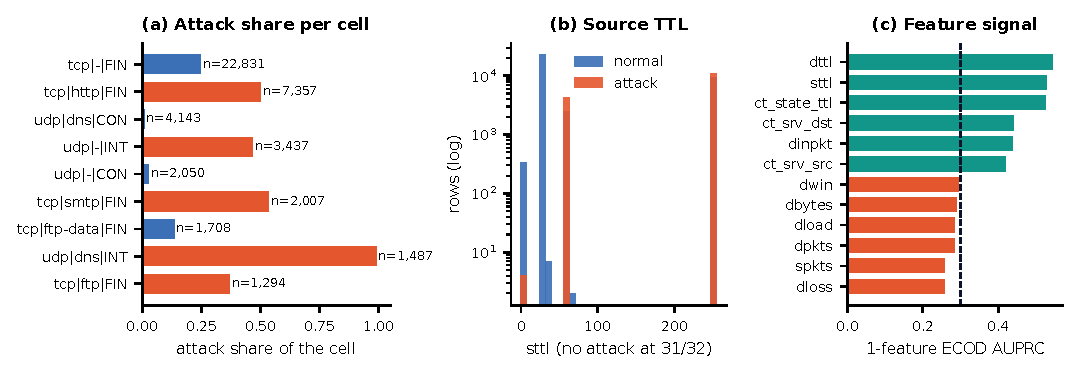
\includegraphics[width=\linewidth]{figs/eda_unsw.pdf}
\caption{UNSW-NB15. (a) Attack share of the nine largest proto$|$service$|$state cells. (b) Source TTL: log counts show normals at 31/32 and no attacks there. (c) The six best and six worst columns by single-feature ECOD AUPRC (teal: above chance, red: below chance; dashed line: base rate 0.30).}\label{fig:edau}\end{figure}

\paragraph{NSL-KDD: strong normals, content features that matter.} Real normals already score 0.929. Figure~\ref{fig:edan} shows that attacks are concentrated in connection types rather than in numeric tails: 63\% of \texttt{logged\_in}=0 rows are attacks but only 1.2\% of \texttt{logged\_in}=1 rows (98.3\% of all attacks are not logged in), flag S0 is 98\% attack, and ICMP 75\%. Several columns carry no signal for ECOD (\texttt{srv\_count} at 0.315 is below the 0.333 base rate, similarly \texttt{srv\_diff\_host\_rate}, \texttt{duration}, \texttt{dst\_host\_count}), while sparse content columns (\texttt{hot}, \texttt{root\_shell}, \dots) show no signal in training but may be the only way to expose content-type attacks in the hidden sets, so they must not be neutralized.

\begin{figure}[t]\centering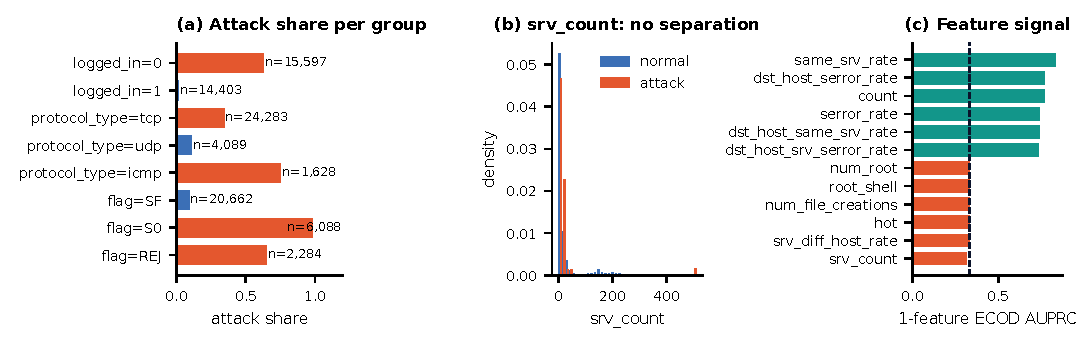
\includegraphics[width=\linewidth]{figs/eda_nsl.pdf}
\caption{NSL-KDD. (a) Attack share by \texttt{logged\_in}, protocol and flag. (b) \texttt{srv\_count} has virtually the same distribution for normals and attacks. (c) Six best and worst columns by single-feature ECOD AUPRC (dashed line: base rate 0.333).}\label{fig:edan}\end{figure}

\paragraph{Engineering implications.} (1) UNSW needs \emph{local} generators (conditioned on the traffic regime), purification of normals that look attack-like, and treatment of columns that mislead. (2) NSL-KDD should keep its real normal modes and only receive targeted corrections. (3) Because the detectors respond to shape, a ``bad'' column is best made uninformative (a flat ECDF) instead of realistic. These three points determine the pipeline below.

% ---------------- 3 Methodology ----------------
\section{Methodology}\label{sec:method}
\subsection{Pipeline overview}
One code path serves both datasets (Figure~\ref{fig:pipe}). A stage is switched off by a neutral parameter (weight scale 0, stretch factor 1, no jitter), never by separate code; Table~\ref{tab:cfg} lists the settings.

\begin{figure}[t]\centering
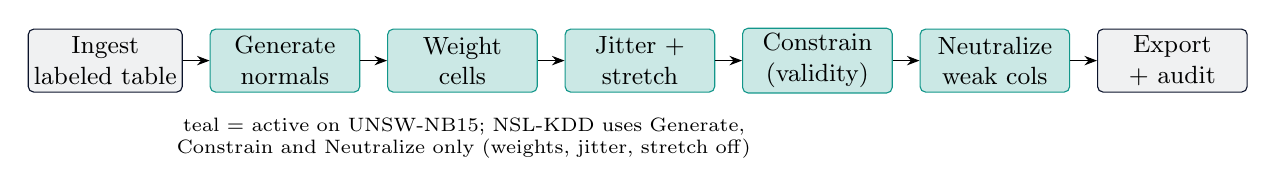
\begin{tikzpicture}[font=\small,node distance=3.4mm,
 st/.style={draw=navy,fill=navy!6,rounded corners=2pt,minimum height=8mm,minimum width=19mm,align=center,inner sep=2pt},
 on/.style={st,fill=teal!22,draw=teal},off/.style={st,fill=gray!12,draw=gray!60,text=gray!70!black}]
\node[st](a){Ingest\\labeled table};
\node[on,right=of a](b){Generate\\normals};
\node[on,right=of b](c){Weight\\cells};
\node[on,right=of c](d){Jitter +\\stretch};
\node[on,right=of d](e){Constrain\\(validity)};
\node[on,right=of e](f){Neutralize\\weak cols};
\node[st,right=of f](g){Export\\+ audit};
\foreach\x/\y in {a/b,b/c,c/d,d/e,e/f,f/g}{\draw[-{Stealth[length=1.6mm]}](\x)--(\y);}
\node[below=2mm of c,font=\scriptsize,text width=9cm,align=center]{teal = active on UNSW-NB15;\ NSL-KDD uses Generate, Constrain and Neutralize only (weights, jitter, stretch off)};
\end{tikzpicture}
\caption{The shared pipeline. Final audit: row count, schema order, NaN/Inf, unique IDs, constraint violations, comparison with a reference file.}\label{fig:pipe}\end{figure}

\begin{table}[t]\centering\small
\begin{tabular}{P{2.0cm}P{6.7cm}P{6.7cm}}\toprule
Stage & UNSW-NB15 (70\,000 rows) & NSL-KDD (40\,000 rows)\\\midrule
Generate & one contrastive-DVS Gaussian copula conditioned on joint proto$|$service$|$state; $\alpha{=}35$, $\tau_{u}{=}0.15$, $\tau_{low}{=}0.05$, 5 bags & 19\,600 scrubbed real normals + 20\,400 copula rows from SILK-style k-FreqItems clusters ($k{=}20$, centre frequency 0.35, min.\ cluster 500, tail slack 1.05)\\
Weight & cell weights $\exp(3\theta_c)$ on 14 cells, resample with replacement & off\\
Jitter / stretch & $0.10\sigma$ noise on repeated rows; $10\times$ stretch of the tail opposite to attacks on 4 gated columns & off\\
Constrain & non-negativity, integer counts, TTL in $[0,255]$, non-TCP zeroing, $\textit{tcprtt}=\textit{synack}+\textit{ackdat}$ & rates in $[0,1]$, counts non-negative, binary flags, no \texttt{root\_shell} when not logged in\\
Neutralize & uniform$[q_{01},q_{99}]$ on 4 columns: \texttt{sinpkt}, \texttt{sjit}, \texttt{ct\_dst\_src\_ltm}, \texttt{ct\_dst\_ltm} & uniform$[q_{01},q_{99}]$ on 6 columns: \texttt{srv\_count}, \texttt{srv\_diff\_host\_rate}, \texttt{duration}, \texttt{dst\_host\_count}, \texttt{dst\_host\_same\_src\_port\_rate}, \texttt{dst\_host\_rerror\_rate}\\
Caps & \texttt{ct\_*\_ltm} $\le100$, \texttt{dmean} $\le1500$ & none\\\bottomrule
\end{tabular}
\caption{Final configuration of the common pipeline (\texttt{final\_pipeline/config.py}).}\label{tab:cfg}\end{table}

\subsection{UNSW-NB15 generator: contrastive DVS copula}
\textbf{Utility.} For each numeric feature $j$ we fit ECOD on that column of the normals and score all training rows; $c_j=\mathrm{Corr}(s^{\mathrm{ECOD}}_j(X),y)$ measures how much the feature separates attacks. Features with $c_j>\tau_u=0.15$ form the high-utility set $H$.\\
\textbf{Purification.} A real normal that looks like an attack on the useful features is a liability: the detector would learn to treat attack-like values as normal. We give each normal $i$ the weight
\begin{equation}
w_i\;\propto\;\exp\!\Big(\sum_{j\in H}\big[\log p_0(x_{ij})-\log p_1(x_{ij})\big]\Big),
\end{equation}
with $p_0,p_1$ the per-feature densities of normals and attacks, so normals that are more likely under the attack density are sampled less.\\
\textbf{Conditioned copula.} We fit a Gaussian copula (empirical marginals, rank correlation) on the weighted normals \emph{per group} and shrink each group's correlation matrix toward the global one,
$R^{*}_g=\lambda_g R_g+(1-\lambda_g)R_0$ with $\lambda_g$ increasing in group size (empirical Bayes). The group is the joint \texttt{proto}$|$\texttt{service}$|$\texttt{state} cell, so a generated row stays inside one traffic regime.\\
\textbf{Dispersion.} Low-utility continuous columns ($c_j<\tau_{low}=0.05$) are widened, $\sigma^{\mathrm{DVS}}_j=\alpha\,(\tau_{low}-c_j)_+\sigma_j$ with $\alpha=35$, so that they become flat and uninformative. Integer, structural and high-utility columns stay within the observed normal range. Five bags with different seeds are concatenated.

\subsection{UNSW-NB15 post-processing}
\textbf{Category-cell weights.} Rows are resampled with replacement with probability proportional to $\exp(3\theta_c)$, where the 14 weights $\theta_c$ over proto/service/state cells were fitted by an evolution-strategy search against the harness. They shift mass away from the attack-overlapping tcp cells (multipliers 0.57 for tcp$|-|$FIN, 0.35 for tcp$|$http$|$FIN, 0.06 for tcp$|$ftp$|$FIN). The fitted weights do not track the attack/normal ratio of the cells (Spearman $0.03$).\\
\textbf{Duplicate jitter.} Weighted resampling repeats rows; only the repeats receive $\mathcal N(0,(0.10\sigma_j)^2)$ noise on 11 continuous columns, bounded below by the observed minimum.\\
\textbf{Gated tail stretch.} Attacks are clustered (KMeans, 4 clusters, standardized log space). A column is stretched only if its attack-vs-normal AUC is at least 0.58 \emph{and} the attack direction agrees in at least 75\% of the clusters (\texttt{dload}, \texttt{dmean}, \texttt{ct\_dst\_ltm}, \texttt{ct\_src\_ltm}). The \emph{opposite} normal tail is expanded $10\times$. The detectors then see more normal mass beyond the normal range on the side that attacks never occupy, which lowers the scores of legitimate high-valued normals without touching the attack-side tail (a mechanistic reading, supported by the small but consistent gain).\\
\textbf{Constraints vs.\ neutralization.} Constraints restore \emph{validity} (fixed domain rules, applied everywhere an invalid value occurs). Neutralization deliberately \emph{removes information}: selected columns are replaced by independent draws from $U[q_{01},q_{99}]$ of the normals. A uniform column has a linear ECDF (flat for ECOD) and wastes IForest's random splits (Figure~\ref{fig:shape}). The four UNSW columns come from a stability-gated leave-one-fold-out harness (selected only if the gain is stable across folds); caps keep stretched \texttt{ct\_*} and \texttt{dmean} physically valid.

\begin{figure}[t]\centering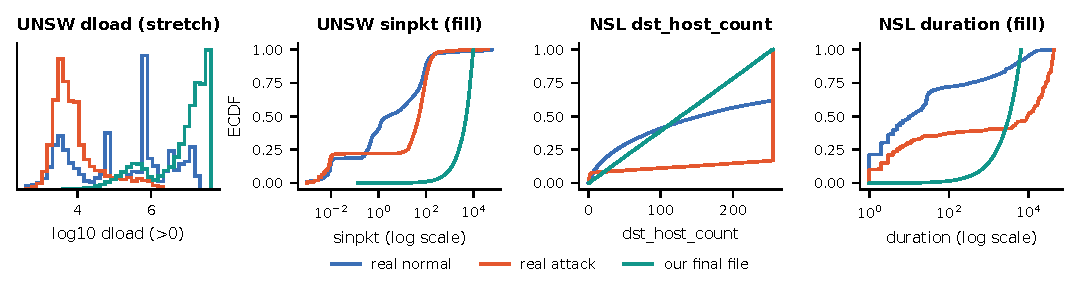
\includegraphics[width=\linewidth]{figs/shaping.pdf}
\caption{What shaping does to marginals (real normals, real attacks, and our final file). Tail stretch moves normal mass to large \texttt{dload}; uniform fill replaces \texttt{sinpkt}, \texttt{dst\_host\_count} and \texttt{duration} by a near-linear (flat-density) ECDF, which is deliberately unrealistic.}\label{fig:shape}\end{figure}

\subsection{NSL-KDD generator and neutralization}
Because real NSL normals are already strong, we \emph{keep} 19\,600 of the 20\,000 normals (a 2\% Isolation-Forest scrub) and add 20\,400 generated rows. Rows are tokenized as itemsets (categorical values exact, low-cardinality integers exact, continuous values in five quantile bins). MinHash (48 hashes, 12 LSH bands)~\cite{minhash} finds similar-row buckets whose frequent tokens act as sparse centres; k-means++-style seeding~\cite{kmpp} on weighted Jaccard similarity picks $k=20$ separated seeds, and k-FreqItems iterations (Jaccard distance, frequency-based centre updates) refine the clusters (16 non-trivial clusters in the winning run, each $\ge500$ rows). A Gaussian copula with tail slack 1.05 is fitted inside each cluster and rows are allocated in proportion to cluster size. Jaccard similarity avoids imposing a Euclidean metric on categorical attributes. This generator is from teammate V.\ Rao's branch and is vendored unmodified.\\
\textbf{Neutralization.} Non-sparse columns whose single-feature ECOD lift is at most 0.10 are uniform-filled; \texttt{dst\_host\_srv\_diff\_host\_rate} is excluded because filling it lost 0.0014 on the leaderboard. Sparse content columns are protected by a support guard.

% ---------------- 4 Experiments ----------------
\section{Experiments and Results}\label{sec:exp}
\paragraph{Protocol.} Variants were ranked on the public leaderboard (before the reveal). We use these pre-reveal public scores for all ablations. A local 14-fold shift-aware harness (leave-one-attack-cluster-out, unseen category groups, tail folds, combinations) pre-screened ideas. After the hidden data were revealed the leaderboard was re-scored on a different scale; we therefore compare variants only \emph{within} each scale (Table~\ref{tab:final} reports the final scale).

\subsection{What worked: the progression}
Figure~\ref{fig:journey} and Table~\ref{tab:uns} show the cumulative UNSW result. Table~\ref{tab:nsl} shows NSL-KDD. Each row changes one thing relative to the row before it, unless noted.

\begin{figure}[t]\centering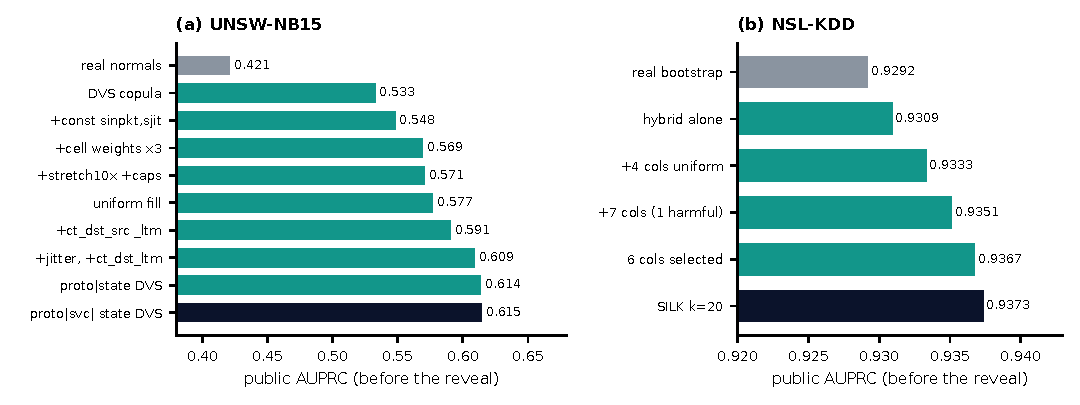
\includegraphics[width=\linewidth]{figs/journey.pdf}
\caption{Public AUPRC before the reveal for the cumulative improvements (grey: real normals; teal: intermediate steps; navy: final defaults).}\label{fig:journey}\end{figure}

\begin{table}[t]\centering\small
\begin{tabular}{p{7.8cm}rr}\toprule
Step (UNSW-NB15) & Public AUPRC & $\Delta$\\\midrule
Bootstrap of real normals & 0.4210 & --\\
Contrastive DVS copula, proto-conditioned & 0.5326 & +0.1116\\
+ stability-gated constants (\texttt{sinpkt}, \texttt{sjit}) & 0.5480 & +0.0154\\
+ cell weights $\times1/\times2/\times3/\times4$ & 0.5547/0.5625/\best{0.5694}/0.5611 & +0.0214\\
+ $10\times$ stretch with physical caps & 0.5707 & +0.0013\\
uniform instead of constant fill & 0.5770 & +0.0063\\
+ \texttt{ct\_dst\_src\_ltm} filled (selection re-run) & 0.5907 & +0.0137\\
+ duplicate jitter, + \texttt{ct\_dst\_ltm} (rounds 1--2) & 0.6091 & +0.0184\\
50\% proto + 50\% state DVS (teammate) & 0.6132 & +0.0041\\
single DVS on joint proto$|$state & 0.6139 & +0.0008\\
\best{single DVS on joint proto$|$service$|$state (final)} & \best{0.6145} & +0.0006\\\bottomrule
\end{tabular}
\caption{UNSW-NB15 cumulative ablation (pre-reveal public scores).}\label{tab:uns}\end{table}

\begin{table}[t]\centering\small
\begin{tabular}{p{9.5cm}rr}\toprule
Step (NSL-KDD) & Public AUPRC & $\Delta$\\\midrule
Bootstrap of real normals & 0.9292 & --\\
Hybrid (real + itemset-cluster copulas) alone & 0.9309 & +0.0017\\
+ 4 uniform-filled columns & 0.9333 & +0.0024\\
+ 7 columns (includes one harmful column) & 0.9351 & +0.0018\\
6 columns (harmful column removed) & 0.9367 & +0.0016\\
\best{SILK-seeded k-FreqItems clusters instead of itemset clusters} & \best{0.9373} & +0.0006\\\bottomrule
\end{tabular}
\caption{NSL-KDD cumulative ablation (pre-reveal public scores). The last step is within noise.}\label{tab:nsl}\end{table}

\begin{figure}[t]\centering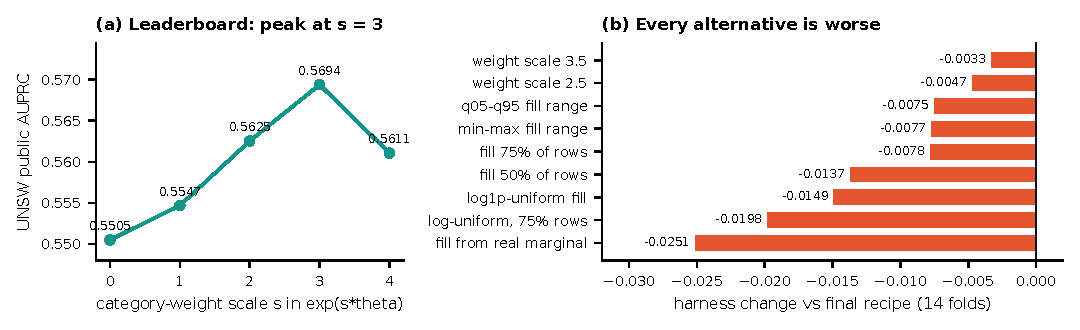
\includegraphics[width=\linewidth]{figs/sensitivity.pdf}
\caption{Sensitivity around the final UNSW recipe. (a) Leaderboard AUPRC against the cell-weight scale (6$\times$ stretch base): a sharp peak at $s=3$. (b) Harness change from the final recipe for alternative fill ranges, fill fractions, fill shapes and weight scales; none improves on it.}\label{fig:sens}\end{figure}

\textbf{Reading the results.} \emph{UNSW:} purification plus conditioned generation is the large step (+0.11 over real normals before any post-processing; in the harness, removing purification costs 0.075 AUPRC, 0.4960 vs 0.5704). Every later stage adds between 0.001 and 0.02, and several of them combine super-additively (selection round 3 and jitter gave $+0.0308$ vs.\ $+0.0248$ expected). The conditioning ladder (proto $\to$ proto$|$state $\to$ proto$|$service$|$state) shows diminishing returns. \emph{NSL-KDD:} everything beyond keeping the real normals adds a total of only 0.0082, mostly from uniform-filling six columns; the data were close to a ceiling.

\subsection{Final result on the hidden data}
Table~\ref{tab:final} gives the scores of the two selected files (the pre-reveal best files, as required). Scores are on the final evaluation scale and are not comparable with the pre-reveal public scores. The final scores are higher in absolute terms, but because the scale changed we do not read this as evidence about overfitting or generalization. After the reveal, two non-selected variants (35\% state share on UNSW; $k=18$, centre frequency 0.30 on NSL-KDD) scored 0.68651 and 0.95276, which are 0.0014 and 0.0003 above our final files.
\begin{table}[h]\centering\small
\begin{tabular}{lrrr}\toprule
Dataset & Pre-reveal public (selected file) & Final hidden-test AUPRC & Selected configuration\\\midrule
UNSW-NB15 & 0.61452 & \best{0.68508} & single DVS, proto$|$service$|$state\\
NSL-KDD & 0.93734 & \best{0.95247} & SILK k-FreqItems $k{=}20$, cf 0.35\\\bottomrule
\end{tabular}
\caption{Selected submissions. The two score columns use different scales.}\label{tab:final}\end{table}

\subsection{What did not work, and why}
Table~\ref{tab:neg} lists the negative results; each has a cause we could check or at least argue for. The pattern is that anything that makes the data ``more realistic'', ``more balanced'' or ``more complex'' lost, while anything that made the detector's job easier won.

\begin{table}[!t]\centering\small
\begin{tabular}{P{3.8cm}P{1.6cm}P{1.5cm}P{8.2cm}}\toprule
Experiment & NSL-KDD & UNSW-NB15 & Why it failed\\\midrule
CTGAN~\cite{ctgan} & 0.9215 & 0.3925 & Optimizes fidelity; sparse categories and detector-relevant tails are not preserved; UNSW is worse than real normals\\
Global clustering + copula & 0.9281 & 0.4397 & Cluster objective misaligned with detector utility\\
Density-ratio rejection & 0.9279 & 0.4925 & Hard rejection over-contracts the normal support and removes useful normal modes\\
DVS purification applied to NSL-KDD & $\approx$0.899 & -- & Over-purifies normals that are already strong; NSL needs preservation\\
Constant fill of 11 columns (NSL) & 0.9180 & -- & Froze informative columns (\texttt{service}, \texttt{logged\_in}); the sparse-support guard prevents this\\
Category weights $\pm0.5$ (NSL) & 0.922/0.929 & -- & Weights on service/flag distort useful normal proportions; no signal lever\\
Log-uniform fill (NSL) & 0.9310 & -- & Uniform on the raw scale (0.9367) is better; compresses the range the detector sees\\
Adding \texttt{dst\_host\_srv\_\allowbreak diff\_host\_rate} (NSL) & 0.932 & -- & Filling it lost 0.0014 although its single-feature lift is only 0.036: lift alone is not sufficient evidence\\
(protocol, flag) partition (NSL) & 0.936/0.937 & -- & No gain over SILK; the flag partition adds nothing\\
No duplicate rows (16$\times$ pool, no replacement) & -- & 0.5663 & Likely because resampling with replacement keeps more mass on useful cells; removing duplicates lost 0.0044\\
40-cell weights fitted on a different base & -- & 0.5939 & $-0.0206$: harness gain did not transfer (see Table~\ref{tab:har})\\
Extra $\times0.5$ on four shared cells & -- & 0.5975 & $-0.0171$: both directions lose, the 14-cell optimum is sharp\\
Three-way mix (proto, state, SILK) & -- & 0.6078 & More partitions than two is worse than one or two\\
65\% state-conditioned DVS & -- & 0.6097 & Protocol structure is under-represented\\\bottomrule
\end{tabular}
\caption{Negative results (pre-reveal public AUPRC).}\label{tab:neg}\end{table}

\subsection{Where the remaining error sits, and how reliable was our validation?}
\begin{minipage}[t]{0.52\linewidth}\vspace{0pt}
\textbf{Attack clusters.} Training the detectors on our final UNSW file and scoring the real training rows (in-sample, AUROC of each attack cluster against all normals) lifts the \texttt{tcp|http|FIN} cluster from 0.72 to 0.94 and the large TCP cluster C3 (54.5\% of attacks) from 0.50 to 0.78, but \emph{lowers} the \texttt{udp|INT} cluster from 0.91 to 0.83 (Figure~\ref{fig:clu}). A supervised classifier reaches 0.97 within C3's cell but unsupervised views top out at 0.75--0.80: only 33\% of C3's attacks fall outside the cell normals' $[q_{01},q_{99}]$ on any column, so most sit inside the normal bulk and no tail shaping can separate them. Our pool also contains no \texttt{udp|-|INT}, \texttt{tcp|-|REQ} or ARP normals (about 8\% of the real normals).
\end{minipage}\hfill
\begin{minipage}[t]{0.45\linewidth}\vspace{0pt}
\centering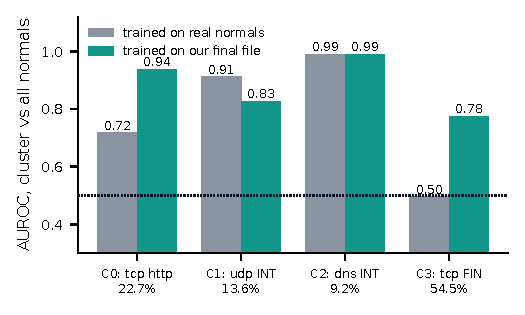
\includegraphics[width=\linewidth]{figs/clusters.pdf}
\captionof{figure}{AUROC of each attack cluster vs.\ all normals (in-sample, UNSW).}\label{fig:clu}
\end{minipage}

\medskip
\textbf{Validation harness vs.\ leaderboard.} Table~\ref{tab:har} compares what the harness predicted with what the leaderboard returned. The harness tracks UNSW within about 0.02 and found the right peak of the weight scale ($\times3$) and the right columns to fill; it mis-ranked finer category weights, could not tell generator variants apart, and was anti-informative on NSL-KDD.

\begin{table}[h]\centering\small
\begin{tabular}{P{6.6cm}P{3.7cm}P{3.1cm}}\toprule
Decision & Harness prediction & Leaderboard\\\midrule
40-cell category weights vs 14-cell & +0.0069 held-out (+0.0172 in-sample) & $-0.0206$\\
UNSW uniform vs constant fill of \texttt{sinpkt}, \texttt{sjit} & +0.0023 & +0.0063\\
\texttt{ct\_dst\_ltm} added to the filled columns & +0.0037 & +0.0012\\
Duplicate-row jitter ($0.10\sigma$) & +0.0057 & +0.0111\\
50\% proto + 50\% state vs proto-only generator & no difference (0.5704 both) & +0.0041\\
NSL-KDD: hold \texttt{srv\_count}, \texttt{srv\_diff\_host\_rate} constant & $-0.003$ / $-0.0014$ & +0.0009\\
NSL-KDD: log-uniform fill & ($-0.0149$ on UNSW) & $-0.0057$\\\bottomrule
\end{tabular}
\caption{Harness vs.\ leaderboard on individual decisions. Disagreements on weights and NSL fill made the leaderboard the arbiter.}\label{tab:har}\end{table}

% ---------------- 5 Lessons ----------------
\section{Lessons Learned and Discussion}\label{sec:lessons}
\begin{enumerate}[label=\textbf{L\arabic*.},leftmargin=2.0em]
\item \textbf{Shape the data for the detector, not for fidelity.} The fidelity-driven baselines (CTGAN~\cite{ctgan}, global clustering) scored 0.39 and 0.44 on UNSW against 0.42 for a plain bootstrap of the real normals, while deliberately unrealistic choices won: a uniform column beat a constant one (UNSW 0.5770 vs 0.5707, NSL-KDD 0.9309 vs 0.9290), and a fill that copies the real marginal was the worst option (in the harness a quantile fill from the real marginal scored $-0.0251$, 0 of 14 folds improved). For ECOD and IForest the question is what the detectors will see, not whether a row could exist.
\item \textbf{Same recipe, different response, so the datasets need different parameters.} Contrastive purification is worth roughly $+0.075$ on UNSW but applied to NSL-KDD it lowered the score from 0.929 to about 0.899; the category weights are the largest lever on UNSW (a $\pm0.02$ swing) and an empty lever on NSL-KDD. The difference follows the data: UNSW has a dominant attack-free Campus-LAN segment and heterogeneous regimes, NSL-KDD has strong real normal modes and attacks that are separable by connection type. Stages controlled by neutral parameters let one pipeline serve both.
\item \textbf{Locality, not complexity, drives generator quality.} Conditioning on proto, then proto$|$state, then proto$|$service$|$state improved the score monotonically (0.6091 $\to$ 0.6139 $\to$ 0.6145), whereas mixing three partitions or adding SILK clusters to UNSW lost. On NSL-KDD, clusters over mixed-attribute itemsets gave small gains on top of the real normals.
\item \textbf{Local validation is a filter, not an oracle.} The harness was reliable for ranking columns to neutralize on UNSW and for the weight-scale peak, but not for finer weights, generators or any NSL-KDD decision. Fitted weights that looked good in-sample and held-out lost 0.02 on the leaderboard, and we twice built a causal story from a single probe (``upweighted shared cells hurt, so downweight them'') that the next experiment refuted (both directions lost). We now treat mechanisms as hypotheses until an A/B test supports them.
\item \textbf{Sharp optima and small effects.} The 14-cell $\times3$ weights, the $[q_{01},q_{99}]$ fill range and the purification strength each sat at a local optimum; every alternative we tried (more or less weight, other ranges, partial fill, other purification powers) was worse or equal. Differences below about 0.001 are noise on our evidence (e.g.\ SILK $+0.0006$, joint service conditioning $+0.0006$), and we report them as such.
\item \textbf{Remaining headroom is in the hard cluster.} More than half of the UNSW attacks (C3) sit inside the normal bulk and cannot be separated by an unsupervised view of the data; the gap to the supervised ceiling (0.97 vs.\ about 0.80) suggests that further gains need more than shape; restoring the normal regimes that the pool omits is the one untested lever with a signal.
\end{enumerate}

\textbf{Limitations.} Many column decisions were tuned on public scores, and the NSL-KDD and UNSW selectors differ (a leave-one-fold-out harness vs.\ a label-based lift rule), which strains the ``one transferable pipeline'' requirement. Pre-computed artifacts (cell weights, selection tables) are shipped rather than recomputed. Our mechanistic explanations (why the opposite-tail stretch and uniform fill help) are consistent with the data but were not isolated with dedicated experiments. After the reveal the scores moved to a new scale, so we cannot quantify a generalization gap.

\section{Conclusion}
Detector-aware distribution engineering, not generator complexity, was the dominant source of performance. A single six-stage pipeline with per-dataset parameters produces training sets on which the fixed ECOD and IForest detectors reach 0.68508 AUPRC on UNSW-NB15 and 0.95247 on NSL-KDD on the final hidden evaluation. The largest single effect is purifying normals that look attack-like; the rest are small, individually validated refinements, and our negative results show where realism, complexity or over-tuning hurt. Future work includes isolating the stretch and fill mechanisms with controlled experiments, restoring the missing normal regimes, and a selection criterion for neutralization that works for both datasets.

\paragraph{Reproducibility and AI use.} \texttt{python final\_pipeline/pipeline.py unsw|nslkdd} regenerates the submitted files; \texttt{verify.py} checks them against the scored files ($10^{-9}$ relative tolerance). All figures in this report are produced by \texttt{report/figs.py} from the training CSVs and the scored files. The authors directed the methods and experiments and made all submissions. Claude (Anthropic), used through Claude Code, assisted with analysis, code and drafting; the authors reviewed and are responsible for the content.

\begin{thebibliography}{9}\small
\bibitem{ecod} Z.~Li, Y.~Zhao, X.~Hu, N.~Botta, C.~Ionescu, G.~Chen. ECOD: Unsupervised outlier detection using empirical cumulative distribution functions. \emph{IEEE TKDE}, 2022.
\bibitem{iforest} F.~T.~Liu, K.~M.~Ting, Z.-H.~Zhou. Isolation Forest. \emph{IEEE ICDM}, 2008.
\bibitem{nsl} M.~Tavallaee, E.~Bagheri, W.~Lu, A.~A.~Ghorbani. A detailed analysis of the KDD CUP 99 data set. \emph{IEEE CISDA}, 2009.
\bibitem{unsw} N.~Moustafa, J.~Slay. UNSW-NB15: A comprehensive data set for network intrusion detection systems. \emph{MilCIS}, 2015.
\bibitem{ctgan} L.~Xu, M.~Skoularidou, A.~Cuesta-Infante, K.~Veeramachaneni. Modeling tabular data using conditional GAN. \emph{NeurIPS}, 2019.
\bibitem{minhash} A.~Z.~Broder. On the resemblance and containment of documents. \emph{SEQUENCES}, 1997.
\bibitem{kmpp} D.~Arthur, S.~Vassilvitskii. k-means++: The advantages of careful seeding. \emph{SODA}, 2007.
\end{thebibliography}
\end{document}
